\section{Laboratory experiment and results}\label{sec:lab}
\subsection{Specimen and registered ports}
The suspended semi-cylindrical mock-up has a deck, internal frames and
machinery seats, axial length 1.8 m and nominal shell radius 0.45 m
(Fig.~\ref{fig:experiment}). It is tested inverted. Suspension and fixture
stiffness and damping were not independently measured; their nominal
values below are prior assumptions.

Two random shaker inputs at P6 and P8 are measured by interface-force
channels 59 and 60 in newtons. Of 40 acceleration channels in m\,s$^{-2}$,
31 enter fitting, giving 62 transfers. ACC8 and ACC40 are excluded from
fitting and completion selection. Channels 13, 23, 24, 26, 27, 31 and 32
retain the source exclusions for fixture-motion or mapping concerns.

Bilinear FE interpolation and the assigned directions define $S,B$ and the
33 independent rows of $A$. A1--A8 denote ACC33--ACC40, with
photograph-derived positions and assumed $-y$ directions. Older shell
channels use outward normals; deck responses and both forces use $+z$.
Only $y,z$ translations enter this registration. Photograph-derived position
uncertainty is about $\pm0.05$ m; channel ordering, directions, sensitivity
and latency lack independent certification. Recorded engineering units are
used without fitted gains, delays or phase offsets.

\begin{figure}[tbp]\centering
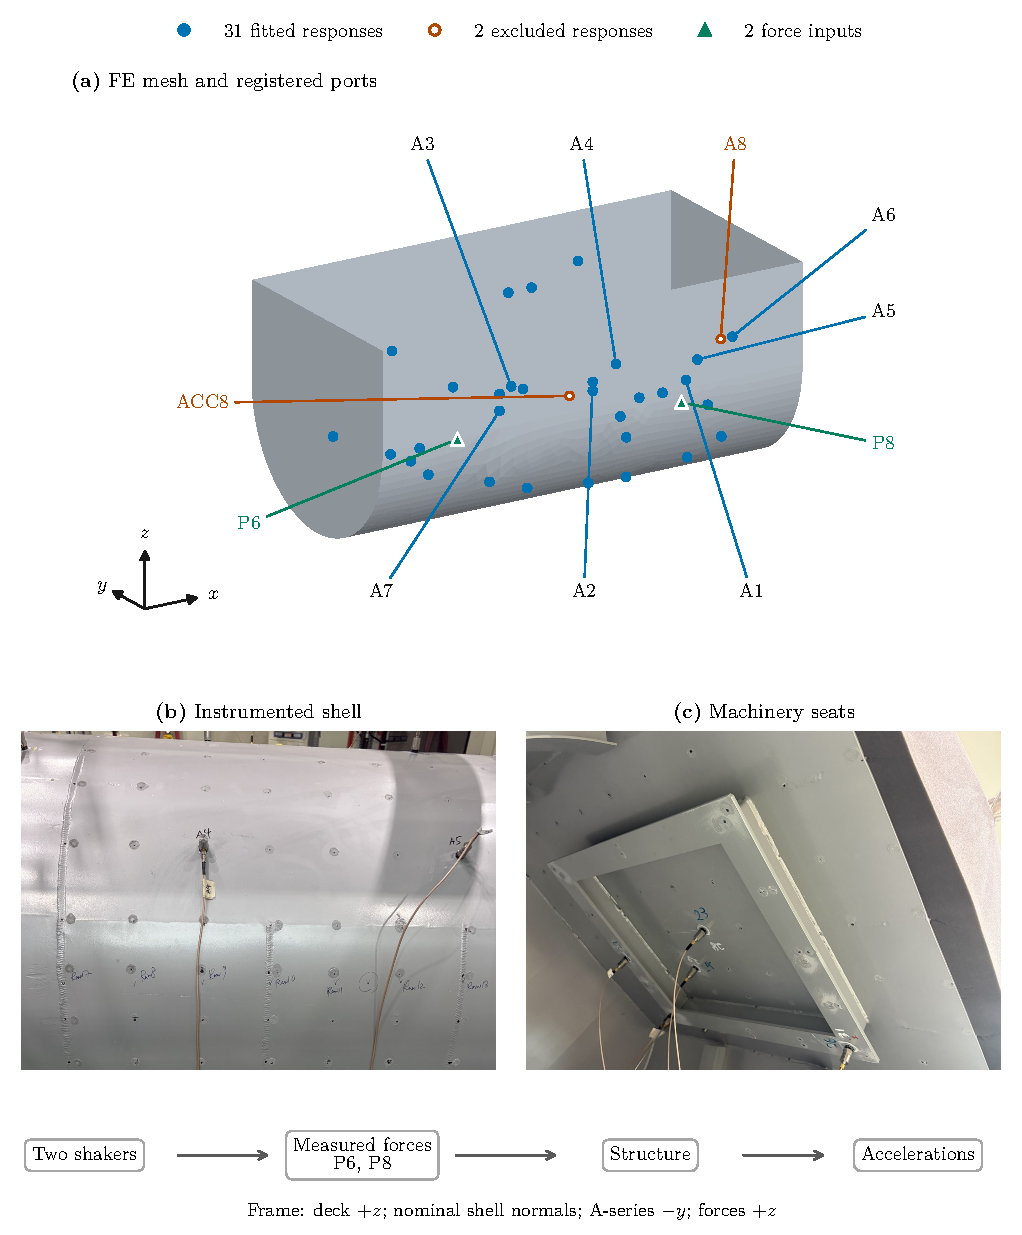
\includegraphics[width=\linewidth]{experimental_overview.pdf}
\caption{Laboratory overview. (a) Registered mesh: blue circles,
fitted responses; open orange circles, excluded ACC8 and A8 (ACC40);
green triangles, P6 and P8. A1--A8 are ACC33--ACC40. (b,c) Preserved
photographs of the inverted specimen and machinery seats. The mesh triad,
not photographic up, defines the coordinate frame.}
\label{fig:experiment}
\end{figure}

\subsection{Acquisition and data roles}
Each record contains 491520 simultaneous samples: 60 s at 8192 Hz.
After mean removal, a degree-two local-polynomial estimator jointly uses
both inputs, a 17-line neighborhood and a record-specific transient
\citep{pintelon2010,pintelon2010b}. Every third center is exported:
\[
 \Delta\nu_{\rm DFT}=1/60\ \mathrm{Hz},\qquad
 \Delta\nu_{\rm FRF}=0.05\ \mathrm{Hz},\qquad
 360\le\nu\le1000\ \mathrm{Hz},\qquad N=12801.
\]
Joint estimation retains the two-input spectral matrix, as in
$\widehat H=\Phi_{af}\Phi_{ff}^{-1}$; plotted entries are not separate
single-input experiments. The records have fixed roles:
\[
 \begin{array}{cl}
 96&\theta\text{ fitting and transfer scales }d_{oi},\\
 101&\text{order selection, continuation monitoring and force-weight selection},\\
 103&\text{development assessment},\\
 104&\text{additional force-estimation assessment (Appendix~\ref{sec:forces})}.
 \end{array}
\]
Records 96, 101, 103 and the excluded responses have historical development
exposure. Excluded-response values select neither completion fields nor
criterion, margin or physical rows. Record 104 was unused in development.

\subsection{Fitted dynamics}
An earlier grid search on five responses selected $r=384$ and damping
bandwidth $b=24$ using record 101: a paired-block bootstrap accepted
candidates within one standard error of the best, then retained the smallest
pair. The 31-response fit keeps these choices and $\alpha=10^{-5}$.
With $A=[S;B^{\top}]$,
\[
 W\in\R^{33\times384},\qquad R_{\rm o}W\in\R^{31\times384},\qquad
 R_{\rm i}W\in\R^{2\times384},\qquad
 \Gamma,\Omega^2\in\R^{384\times384}.
\]
The 768 first-order states specify the chosen order, not proven minimality.
Full-precision factors accompany the paper. Variable projection, reciprocal
scale balancing and a final conditional response solve give
\[
 (\varepsilon_{96},\varepsilon_{101},\varepsilon_{103})
 =(12.73,15.30,15.57)\%.
\]
Each nonlinear comparison used 180 s. The final conditional-gradient
infinity norm is $1.52\times10^{-14}$, but the full-gradient norm is 0.159;
nonlinear optimality is not established.

\subsection{Nominal shell model}
The fixed prior has 3994 nodes, 4008 four-node shell elements and
$n=23964$ degrees of freedom, six per node:
$(u_x,u_y,u_z,\theta_x,\theta_y,\theta_z)$.
Membrane, bending and MITC-type shear terms \citep{bathe1986}, rotary
inertia and a $10^{-3}$ drilling penalty define the element model.
Nominal material constants are Young's modulus 206 GPa, density
7850 kg\,m$^{-3}$ and Poisson ratio 0.3. Thicknesses for bilge, side,
deck, joint, bulkhead and foundation are $(4,4,5,5,5,8)$ mm.
These are supplied assumptions, not recovered specimen properties.

Distributed translational springs of $10^6$ N\,m$^{-2}$ along 3.6 m of
side rails remove the nominal rigid zero modes; no node is fixed. Forty
10 g sensor masses are attached isotropically at the nearest registered
nodes (maximum mapping offset 0.0267 m). Rigid-translation mass checks give
245.971 kg in each Cartesian direction; symmetry and positive-definite
factorization checks accompany the assembly. Damping comes from $\Gamma$;
no nominal viscous damping matrix is available.

The selector $R$ retains 7988 interleaved $y,z$ translations. The remaining
15976 coordinates are statically condensed, then expanded for every
mechanical projection (Appendix~\ref{sec:field-details}). Thus completion
uses the full $M_0,K_0$ with an explicit static assumption for the omitted
coordinates.

\subsection{Completion and realization}
The trial space $\mathcal U$ holds the static deflections under the 33 unit
port forces and $d=384$ port-invisible fields. The fields are the most
compliant ones in the condensed port-null space of dimension $7988-33=7955$,
ranked by stiffness relative to the displayed diagonal mass
(Appendix~\ref{sec:field-selection}). Sparse solves give the static lift $E\in\R^{23964\times33}$ with
$AE=I_{33}$ and the fields $N\in\R^{23964\times384}$ with $AN=0$ and
$N^{\top}M_0N=I_{384}$. Every candidate reads $T=EW+NZ$ with
$Z\in\R^{384\times384}$, and $\dim\mathcal U=417$. Since $\rank W=33$, the
static map $EW$ lacks $384-33=351$ directions. Eq.~\eqref{eq:rank-feasibility}
holds as $384\ge351$. The margin is
$\delta=10^{-3}\sigma_1(REW)=\LabMargin$ kg$^{-1/2}$.

Training record 96 gives the force spectral matrices on 10241 lines of
360--1000 Hz at 0.0625 Hz (Welch, 16 s Hann windows, 50\% overlap) and with
them $\Phi_q$ by Eq.~\eqref{eq:Pi}. Each mode's share of the fitted strain
energy, $\omega_j^2(\Phi_q)_{jj}/\tr(\Omega^2\Phi_q)$, lies between
\LabShareMin\ and \LabShareMax, so every mode is excited. With two shakers,
however, neighbouring modes move together: \LabCorrelatedPairs\ pairs have
correlation above 0.5, the largest \LabCorrelationMax. Combinations that the
test never moves independently are barely constrained by $J_F$.

The equality-only map has $J_F(\theta,T_{\rm LS})=\LabJFLS$, but
$\sigma_{384}(RT_{\rm LS})=\LabLSMinimum$ kg$^{-1/2}$ lies far below
$\delta$, so the margin is active. From the raised start ($J_F=\LabJFStart$)
the iteration meets both residual tolerances after \LabIterations\
iterations (primal \LabPrimalResidual, dual \LabDualResidual) and returns
\[
 J_F(\theta,T_\theta)=\LabJF,\qquad
 \sigma_{384}(RT_\theta)=\LabSigmaMin\ \mathrm{kg}^{-1/2}>\delta,\qquad
 \|VT_\theta-I_{384}\|_F=\LabLeftInverse.
\]
By Theorem~\ref{thm:completion}(iii) the margin costs \LabMarginCost\% of
$J_F$. The port constraint holds to \LabAnchorResidual\ in aggregate and to
\LabWorstPort\ in the worst column. The weakly constrained combinations take
large amplitudes: the nominal mass Gram defect is \LabMassDefect\
(Table~\ref{tab:verification}), against \LabMassDefectJZero\ for the
undamped criterion (Appendix~\ref{sec:completion-benchmark}).

The receptance $\mathcal R_\theta(s)\in\C^{23964\times23964}$ has rank
384 away from its 768 fitted poles. Selecting 384 independent $y,z$ rows
also gives $P=\Pi T_\theta$ and
$\kappa_2(M_\theta)=\LabMassCondition$ for the square realization of
Theorem~\ref{thm:realization}(iii). Predictions use the latent form and
avoid this coordinate-selection conditioning.

\begin{table}[!htbp]\centering
\begin{tabular}{ll}\toprule
Quantity & Primary result\\\midrule
Training / monitoring / development error & 12.73 / 15.30 / 15.57\%\\
$\rank W$ / $\rank T_\theta$ & 33 / 384\\
Hidden fields $d$ & 384\\
$\sigma_r(RT_\theta)$ / margin $\delta$ & 0.08711 / 0.08704\\
$\kappa_2(RT_\theta)$ / $\kappa_2(P)$ & 6092.5 / 86267.0\\
Physical/normalized FRF discrepancy & \ensuremath{2.99\times10^{-9}}\\
\bottomrule\end{tabular}

\caption{Fitted factors and completed map. Singular values of
$RT_\theta$ use unscaled SI translation rows (kg$^{-1/2}$). Numerical rank
uses $10^{-10}\sigma_{\max}$.}
\label{tab:primary}
\end{table}

Registered-transfer preservation is checked at all 12801 frequencies.
The square and latent realizations agree at 41 equally spaced frequencies
to \LabPhysicalResidual\ in aggregate relative norm. State-space displacement,
velocity and acceleration agree within \LabStateResidual\ at five
frequencies, including acceleration feedthrough.

\begin{table}[!htbp]\centering
\begin{tabular}{lr}\toprule
Check & Relative value\\\midrule
Interpolation $AT_\theta=W$ & \ensuremath{1.10\times10^{-15}}\\
Full-band registered FRFs & \ensuremath{6.18\times10^{-12}}\\
Physical force transformation & \ensuremath{2.48\times10^{-15}}\\
Physical response transformation & \ensuremath{1.95\times10^{-14}}\\
Acceleration feedthrough & \ensuremath{2.14\times10^{-13}}\\
Maximum mechanical congruence residual & \ensuremath{6.24\times10^{-10}}\\
Nominal mass Gram defect $\|T_\theta^{\top}M_0T_\theta-I\|_F/\|I\|_F$ & 823.8182\\
Nominal stiffness Gram defect $\|T_\theta^{\top}K_0T_\theta-\Omega^2\|_F/\|\Omega^2\|_F$ & 511.9573\\
\bottomrule\end{tabular}

\caption{Transfer identities and nominal Gram defects. The
last two rows measure nominal incompatibility. They are not numerical
roundoff errors.}
\label{tab:verification}
\end{table}

\subsection{Measured-port assessment}
Across the fitted transfers on record 103, normalized complex errors are
13.87--22.62\% for P6 and 6.06--17.00\% for P8. Median absolute wrapped
phase errors are 3.8--8.7 degrees, including weak-response lines. All 62
transfers retain the training scales.

Figure~\ref{fig:frf-full} shows ACC1, ACC7, ACC15,
ACC21, ACC33 and ACC39, selected at equally spaced ranks in the ordered
fitting-channel list, with all 12801 samples. Eight 20 Hz windows A--H,
one per frequency stratum, are fixed independently of fit quality.

\begin{figure}[tbp]\centering
\captionsetup{skip=2pt}
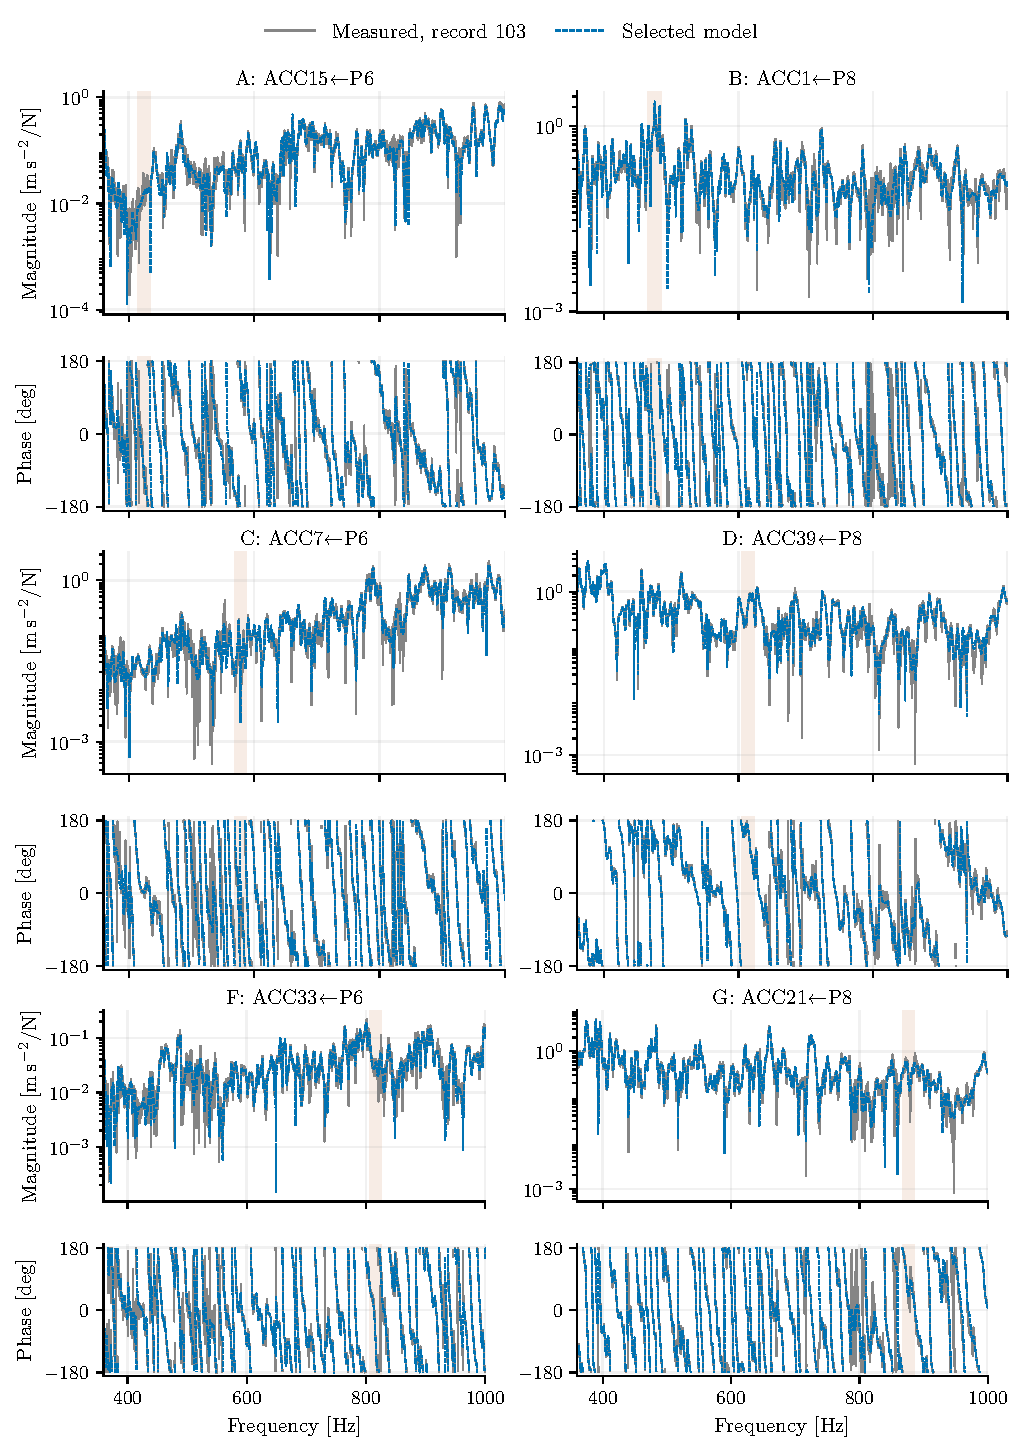
\includegraphics[width=\linewidth]{frf_fullband.pdf}
\caption{Six representative development-record transfers. Grey:
measured. Blue dashed: $H_\theta$. Each cell pairs magnitude and principal
phase. Shading marks fixed 20 Hz windows enlarged in
Fig.~\ref{fig:frf-details-ad}. All 12801 samples are retained.}
\label{fig:frf-full}\label{fig:frf-full-bc}\label{fig:frf-full-df}
\end{figure}

\begin{figure}[tbp]\centering
\captionsetup{skip=2pt}
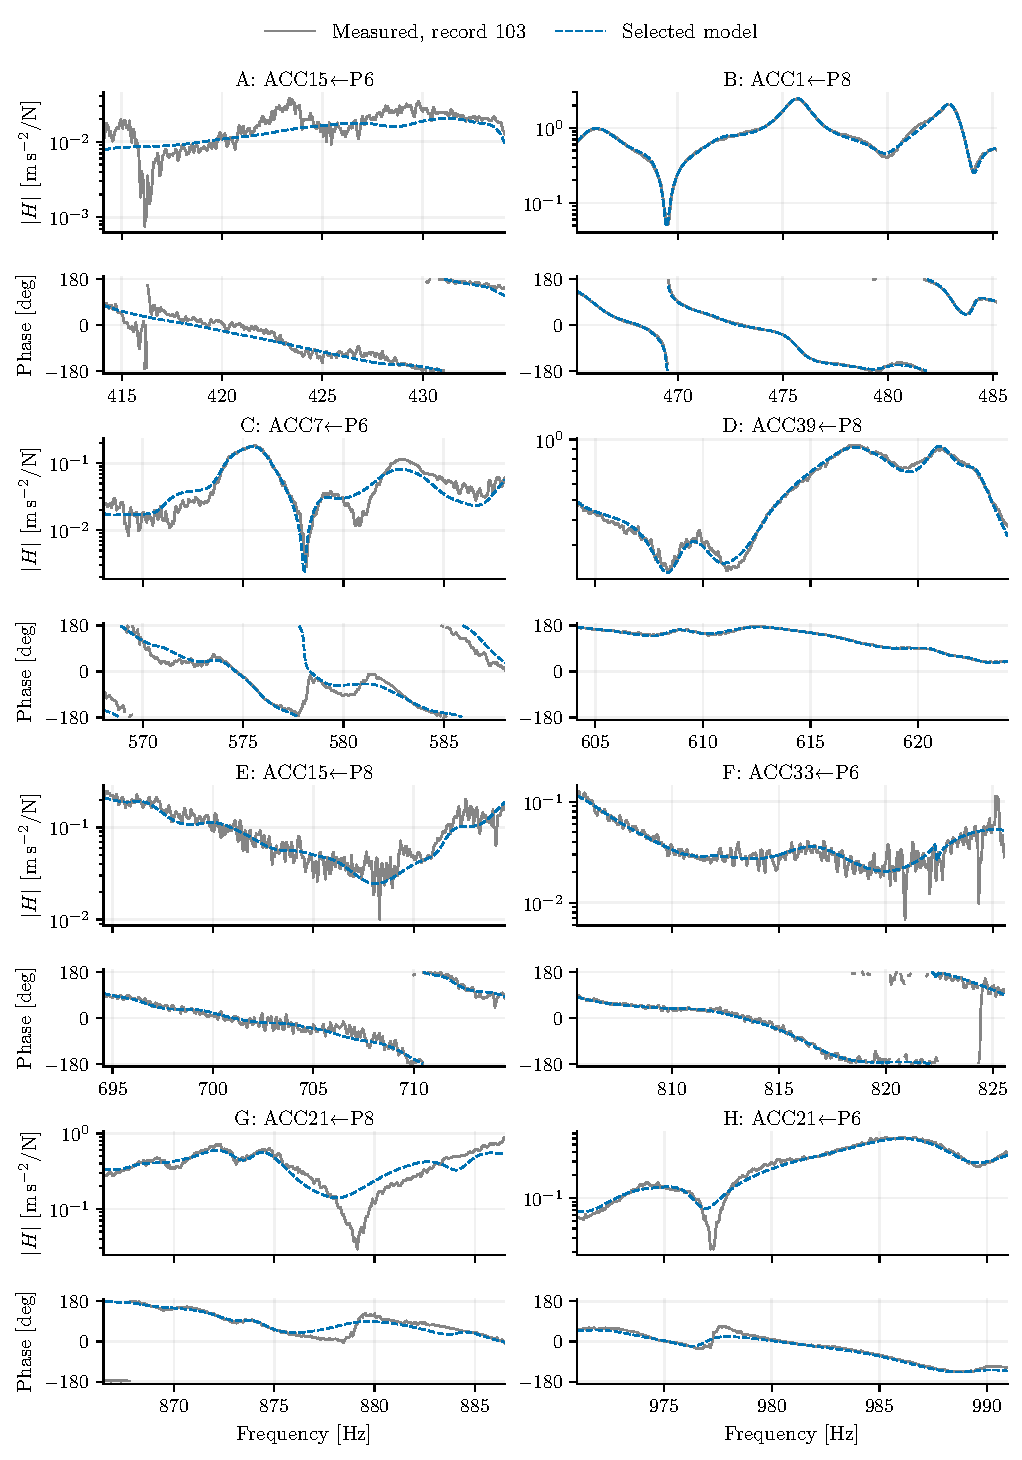
\includegraphics[width=\linewidth]{frf_details_ad.pdf}
\caption{Eight fixed windows A--H on record 103, one per
frequency stratum. Each contains 401 samples over 20 Hz at 0.05 Hz spacing.
Magnitude lies above principal phase in $[-180,180]$ degrees, with gaps
at wraps. No smoothing, unwrapping or plotting gain is applied.}
\label{fig:frf-details-ad}\label{fig:frf-details-eh}
\end{figure}

\subsection{Excluded responses}\label{sec:spatial-results}
For the primary 31-response fit, ACC8 and ACC40 are withheld; let
$S_{\rm c}\in\R^{2\times n}$ denote their registration.
Their completed response coefficients are
\[
 S_{\rm c}T_\theta=S_{\rm c}EW+S_{\rm c}NZ,
\]
so they depend on the hidden fields. The aggregate normalized complex error
is \LabExcludedError\%. ACC8 dominates, and both ACC40 transfers exceed
100\% (Table~\ref{tab:spatial-results}). The undamped criterion gives
\LabExcludedErrorJZero\% (Appendix~\ref{sec:completion-benchmark}). Exact
port preservation and a small nominal residual along the measured motion
therefore do not imply accurate spatial prediction with this prior and
registration.

\begin{table}[!htbp]\centering
\begin{tabular}{lrrr}\toprule
Transfer & Complex error [\%] & RMS error [m\,s$^{-2}$/N] & Median phase error [$^\circ$]\\\midrule
ACC8/P6 & 4281.91 & 4.696 & 88.3\\
ACC8/P8 & 1268.86 & 3.435 & 99.2\\
ACC40/P6 & 244.53 & 0.878 & 77.5\\
ACC40/P8 & 229.71 & 0.989 & 103.8\\
\bottomrule\end{tabular}

\caption{Excluded-response errors on record 103, using the
original training scales. Absolute RMS is the complex accelerance residual.
Phase error is the median absolute wrapped difference, including weak lines.}
\label{tab:spatial-results}
\end{table}

Figure~\ref{fig:spatial-full} shows a second withheld pair, ACC35 and
ACC40, from a separate 30-response refit that excludes ACC8, ACC35 and ACC40
from fitting and completion. The refit starts from the earlier five-response
fit, which also excludes these sensors, and retains order $r=384$, damping
bandwidth $b=24$ and the nominal FE prior. ACC35 is therefore predicted as an
unmeasured response here, although it was fitted in the primary model above.
The pair was chosen among three holdout trials by response-level agreement on
record 101; the displayed record 103 was not used in that choice. On record
103 the normalized complex errors are \FigureEightLeftError\% for ACC35 and
\FigureEightRightError\% for ACC40. Both exceed 100\%, as do the ACC40
transfers of the primary fit.

\begin{figure}[tbp]\centering
\captionsetup{skip=2pt}
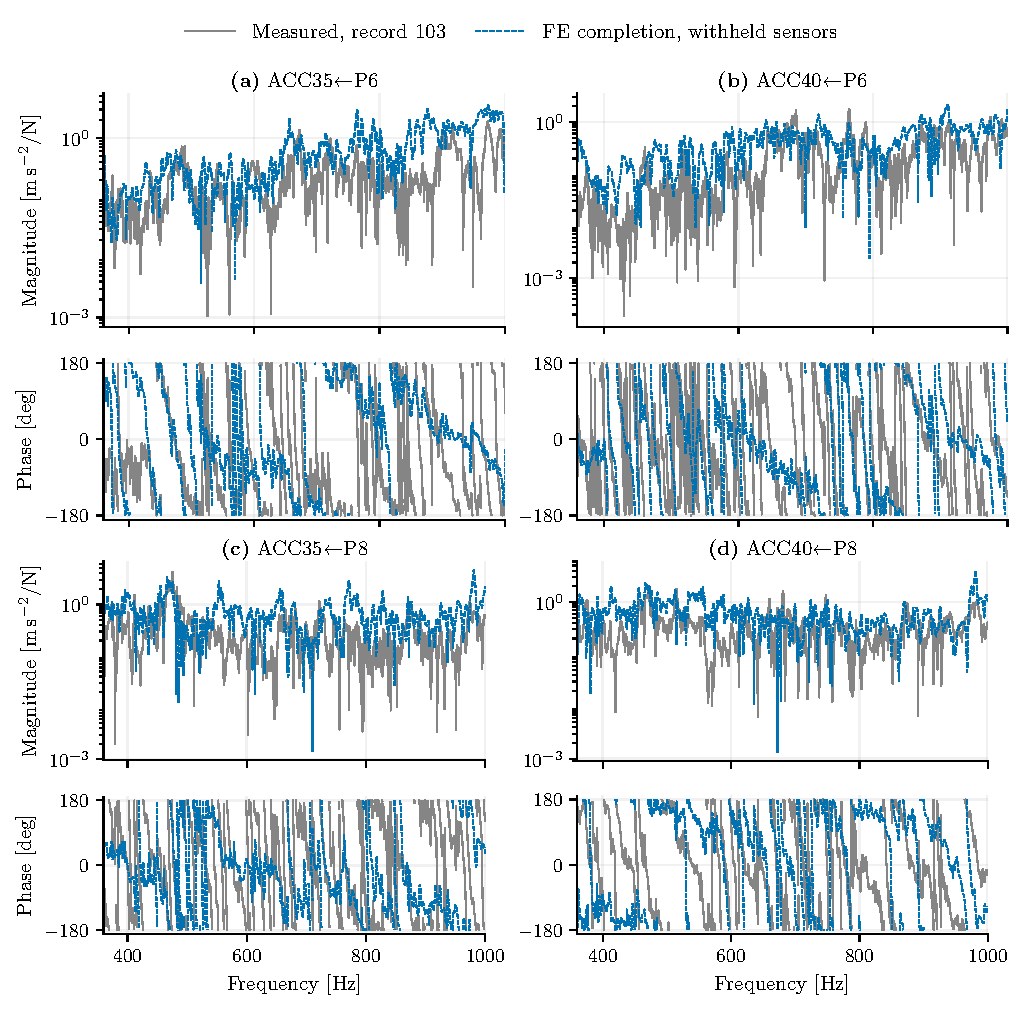
\includegraphics[width=\linewidth]{spatial_fullband.pdf}
\caption{Withheld responses ACC35 (left) and ACC40 (right) on record 103,
from the separate refit that excludes ACC8, ACC35 and ACC40. Top: P6;
bottom: P8. Grey: measured. Blue dashed: completed model. Each cell pairs
magnitude and principal phase. All 12801 samples are retained.}
\label{fig:spatial-full}
\end{figure}
